\documentclass[11pt]{article}

\usepackage[letterpaper,margin=0.82in]{geometry}
\usepackage[T1]{fontenc}
\usepackage[utf8]{inputenc}
\usepackage{lmodern}
\usepackage{microtype}
\usepackage{amsmath,amssymb,mathtools}
\usepackage{booktabs,longtable,tabularx,array}
\usepackage{enumitem}
\usepackage{xcolor}
\usepackage{fancyhdr}
\usepackage{titlesec}
\usepackage[hidelinks]{hyperref}
\usepackage{tikz}
\usetikzlibrary{arrows.meta,positioning,shapes.geometric}
\usepackage[most]{tcolorbox}
\usepackage{lastpage}

\definecolor{predblue}{HTML}{17365D}
\definecolor{softblue}{HTML}{EEF4FA}
\definecolor{softgray}{HTML}{F4F4F4}
\definecolor{softgold}{HTML}{FAF3DF}
\definecolor{softgreen}{HTML}{ECF5EC}
\definecolor{softred}{HTML}{F9EAEA}

\hypersetup{
  pdftitle={Predator ATP: Version Summaries and Design Lineage},
  pdfauthor={Brian Tenneson},
  colorlinks=true,
  linkcolor=predblue,
  urlcolor=predblue
}

\setlength{\parindent}{0pt}
\setlength{\parskip}{0.55em}
\setlist[itemize]{leftmargin=1.4em,itemsep=0.18em,topsep=0.25em}
\setlist[enumerate]{leftmargin=1.7em,itemsep=0.18em,topsep=0.25em}
\titleformat{\section}{\Large\bfseries\color{predblue}}{\thesection.}{0.55em}{}
\titleformat{\subsection}{\large\bfseries}{\thesubsection}{0.5em}{}

\pagestyle{fancy}
\fancyhf{}
\lhead{Predator ATP Version Summaries}
\rhead{Brian Tenneson}
\cfoot{\thepage\ of \pageref{LastPage}}
\setlength{\headheight}{14pt}

\newtcolorbox{statusbox}[1][]{colback=softgray,colframe=black!25,boxrule=0.55pt,arc=1.5mm,left=2.5mm,right=2.5mm,top=1.8mm,bottom=1.8mm,#1}
\newtcolorbox{keybox}[1][]{colback=softblue,colframe=predblue,boxrule=0.7pt,arc=1.5mm,left=2.8mm,right=2.8mm,top=2mm,bottom=2mm,#1}
\newtcolorbox{warningbox}[1][]{colback=softgold,colframe=black!35,boxrule=0.55pt,arc=1.5mm,left=2.5mm,right=2.5mm,top=1.8mm,bottom=1.8mm,#1}

\newcommand{\implemented}{\textbf{Implemented / documented}}
\newcommand{\tested}{\textbf{Implemented and experimentally tested}}
\newcommand{\proposed}{\textbf{Proposed architecture}}
\newcommand{\historical}{\textbf{Historical design stage}}
\newcommand{\Hhat}{\widehat{H}}

\begin{document}

\begin{titlepage}
\thispagestyle{empty}
\vspace*{0.75in}
{\Huge\bfseries\color{predblue} Predator ATP\par}
\vspace{0.12in}
{\LARGE\bfseries Version Summaries and Design Lineage\par}
\vspace{0.20in}
{\large Predator 1 through Predator 8.018, with Predator 9 as the proposed next major generation\par}
\vspace{0.55in}
{\large Brian Tenneson\par}
{\normalsize September 26, 2026\par}
\vfill
\begin{statusbox}
\textbf{Scope.} This reconstruction is based on the surviving Predator papers and reconstruction notes supplied by the author. It preserves the distinction between implemented systems, experimentally measured systems, proposed architectures, and later reconstruction plans. Where the surviving documents do not establish a direct ancestry, the lineage is shown as branching rather than forced into a single linear sequence.
\end{statusbox}
\vfill
\end{titlepage}

\tableofcontents
\newpage

\section{Executive summary}

Predator began as a learned search policy over a small enumerable formal system and gradually moved toward full Metamath proof production, independent certificate verification, learned legal-move ranking, settlement geometry, bounded exactification, and strategy-level self-monitoring.

The design history is best understood through the recurring pattern
\[
\boxed{\text{wall encountered}}
\;\longrightarrow\;
\boxed{\text{new mechanism}}
\;\longrightarrow\;
\boxed{\text{new wall}}.
\]

The surviving documentation supports a high-confidence conceptual reconstruction from Predator 1 through Predator 8.018. The most important distinction in the later line is that Predator 8.004 Dense Closure Distillation is a proposed training/architecture branch and is not established by the surviving documents as a direct ancestor of Predator 8.018.

\begin{keybox}
\textbf{Current implemented endpoint in the surviving reconstruction notes:}
\[
\boxed{\text{Predator 8.018}}
\]
It combines the recovered Predator 8.002 legal proof engine and ML ranker with the 8.015 control modes, the 8.016/8.017 exactification line, and a new resource-aware BAILOUT controller.
\end{keybox}

The proposed next major generation in the present reconstruction is
\[
\boxed{\text{Predator 9: Information-Rich Verified Theorem Search}.}
\]
Predator 9 is not historical source material; it is the current design proposal arising from the reconstructed lineage and the later ATP-information inventory.

\section{Compact lineage table}

\small
\renewcommand{\arraystretch}{1.17}
\begin{longtable}{>{\raggedright\arraybackslash}p{0.11\textwidth} >{\raggedright\arraybackslash}p{0.33\textwidth} >{\raggedright\arraybackslash}p{0.34\textwidth} >{\raggedright\arraybackslash}p{0.13\textwidth}}
\toprule
\textbf{Version} & \textbf{Principal design change} & \textbf{Wall or principal lesson} & \textbf{Status}\\
\midrule
\endhead
Predator 1 & Learned policy over enumerable propositional forward search. & Small fragment makes exhaustive consequence generation possible; does not scale to full set.mm. & Tested \\
Predator 2 & Recasts full-library ATP as premise selection over ZFC/Metamath. & Can rank likely premises but does not construct a proof. & Implemented \\
Predator 3 & Scales the premise-selection pipeline and corpus handling. & Same fundamental limitation: ranking is not proof search. & Implemented \\
Predator 4 & Learned premise ranker over large-scale set.mm reference data. & Strong ranking component, still no inference search. & Tested \\
Predator 5 & Learned state-to-edge search policy trained on BFS-computed geodesics. & Genuine search, but only in a small fragment where BFS ground truth is affordable. & Tested \\
Predator 6 & Expert iteration: use learned policy beyond BFS horizon, then retrain. & Controlled experiment showed no improvement in the chosen fragment; the fragment was too completely priced by BFS. & Tested \\
Predator 7 & Couples large-library ranking to proof search; extracts grammar from Metamath syntax axioms. & One-way matching fails on undetermined assertions such as modus ponens and syllogism. & Implemented \\
Predator 7.1 & Replaces matching with unification and metavariables; emits independently checked certificates. & The ranker was lost in the rewrite, and demonstrated successes were duplicate/instance lookups rather than substantive new proofs. & Tested \\
8.001 & Frozen formal proof engine retained in the recovered 8.x runtime. & Exact transition from 7.1 is not completely documented in the supplied material. & Recovered \\
8.002 & Recovered legal proof engine plus ML legal-move ranker; later serves as native search mode. & Needs higher-level control and trustworthy progress diagnostics. & Recovered \\
8.003 & Broad historical learned model / transfer experiment. & Sparse local semigroup signal plus a legal-candidate filtering defect. & Tested branch \\
8.004 DCD & Dense Closure Distillation: broad pretraining plus bounded verified local closure, policy/value training, readiness gate. & Explicitly proposed as a separate experimental condition; direct ancestry into 8.018 is not established. & Proposed branch \\
8.015 & Adds ATTENTION, SURGE, TORPOR and limited settlement-score influence. & Estimated horizon can appear near settlement without certification. & Implemented \\
8.016 & Adds bounded local BFS exactification around apparently promising states. & Probe was tied to the engine-selected open goal and could miss full local geometry. & Implemented \\
8.017 & Exactification branches over all current open goals and compatible unifying candidates. & Local shell explosion remains; exactification itself needs a resource budget. & Implemented \\
8.018 & Adds self-aware BAILOUT: bounded basin resource tranche, failure memory, basin blacklisting, frontier pruning, deliberate SURGE after bailout. & Still uses non-authoritative approximate progress signals; strategy utility remains crude. & Current implemented endpoint \\
8.019 & Selective kitchen-sink proposal: adaptive utility, SATURATE versus BAILOUT, basin portfolio. & Proposed rather than implemented in the surviving notes. & Proposed \\
Predator 9 & Information-rich verified search using explicit online information state and higher-level allocation control. & Present next-generation proposal, not historical implementation. & Proposed next major version \\
\bottomrule
\end{longtable}
\normalsize

\section{The early line: learning what to search}

\subsection{Predator 1 - learned forward search}

\begin{statusbox}\tested\end{statusbox}

Predator 1 is the original trainable theorem prover. It operates over a small propositional formal system where direct consequences can actually be enumerated. Brute force adds every direct consequence at a stage; Predator scores the available consequences and keeps only the most promising few.

Its central experimental lesson is methodological. Search efficiency cannot be reported without solve rate, because a prover that gives up immediately uses almost no expansions. Predator 1 therefore develops the paired evaluation idea: measure both success and search effort.

\textbf{Contribution to the lineage:}
\begin{itemize}
\item learning can alter search order rather than theoremhood;
\item expansions provide a hardware-independent search-effort measure;
\item temporal splits prevent a model from training on the future;
\item depth remains an intrinsic floor even when breadth is reduced.
\end{itemize}

\textbf{Wall:} the formal fragment is small enough to enumerate, so the approach does not directly transfer to full Metamath ZFC.

\subsection{Predator 2 - premise selection over ZFC}

\begin{statusbox}\implemented\end{statusbox}

Predator 2 responds to the scaling wall by changing the problem. Rather than trying to re-derive all consequences in set.mm, it uses the fact that Metamath proofs explicitly name the axioms and earlier theorems they cite. The machine therefore asks:
\[
\text{Given a target, which available theorems are likely to be used in its proof?}
\]

This converts proof search into a large-library retrieval/ranking problem. Recall and effort become natural metrics: a selector must retrieve the true premises, but should not need to read the entire preceding library to do so.

\textbf{Wall:} Predator 2 ranks premises but cannot build a proof.

\subsection{Predator 3 - premise selection at scale}

\begin{statusbox}\implemented\end{statusbox}

Predator 3 retains the premise-selection objective but improves corpus handling and scale. In the surviving history appendix it is described as the same essential task with engineering made to scale.

\textbf{Wall:} scaling the ranker does not solve the deeper problem. A ranked list is still not a proof.

\subsection{Predator 4 - learning to rank premises}

\begin{statusbox}\tested\end{statusbox}

Predator 4 is the mature premise-ranking component of the early line. It trains a learned ranker on large numbers of logical references from set.mm and evaluates recall-at-$k$ and effort across corpus sizes.

This version is important because its ranker later becomes one of the two components Predator 7 tries to unite: Predator 4 contributes large-library relevance, while Predator 5 contributes actual proof-state search.

\textbf{Wall:}
\[
\boxed{\text{good premise ranking} \neq \text{proof construction}.}
\]

\section{The search-policy line: learning where to move}

\subsection{Predator 5 - search policy from computed geodesics}

\begin{statusbox}\tested\end{statusbox}

Predator 5 is a conceptual pivot. The question changes from
\[
\text{Which library theorem is relevant to the goal?}
\]
to
\[
\text{From proof state }p,\ \text{which legal one-step extension moves toward a shortest proof?}
\]

Training labels are no longer read from human proof histories. Instead, BFS is run first on a small enough fragment to obtain exact graph distances. Every edge lying on some shortest path is a positive action; alternative legal edges at the same state are negatives.

This produces two durable design principles:
\begin{enumerate}
\item \textbf{State-local negatives.} A search policy must rank legal alternatives actually available at the same state.
\item \textbf{Computed labels.} A human proof is only an upper bound on shortest proof length; it does not reveal the rejected frontier.
\end{enumerate}

Predator 5 also clarifies the difference between reordering and pruning. Reordering all admissible moves preserves proof coverage; truncating the move set can destroy completeness.

\textbf{Wall:} exact geodesic labels require BFS to finish, restricting the experiment to a small fragment rather than full set.mm.

\subsection{Predator 6 - expert iteration}

\begin{statusbox}\tested\end{statusbox}

Predator 6 tries the natural next step: train on BFS-certified geodesics, let the policy reach targets beyond the BFS-labelled region, then retrain from the newly reached experience.

The controlled experiment did not improve performance in the chosen fragment. The documented interpretation is not that expert iteration is intrinsically useless, but that the fragment was already completely priced by BFS. There was little meaningful frontier left for expert iteration to discover.

\textbf{Lineage lesson:} a negative experiment can be structurally informative. A learning mechanism must be tested in a regime where its supposed advantage can actually exist.

\section{The Metamath proof-producing line}

\subsection{Predator 7 - ranking coupled to full-corpus search}

\begin{statusbox}\implemented\end{statusbox}

Predator 7 attempts to bridge the Predator 4 and Predator 5 worlds:
\[
\boxed{\text{large-library ranking}} + \boxed{\text{proof-state search}}.
\]

The missing infrastructure is parsing. A Metamath statement is a flat token sequence, so Predator 7 reconstructs syntax from the grammar rules already present in set.mm. This makes proof-state structure explicit enough for search.

\textbf{Wall:} Predator 7 uses one-way matching. This works only when an assertion is determined by its conclusion. Important rules such as modus ponens have hypothesis variables not fixed by the conclusion, so matching alone cannot instantiate them.

\subsection{Predator 7.1 - unification, metavariables, and certificates}

\begin{statusbox}\tested\end{statusbox}

Predator 7.1 replaces one-way matching with unification over two namespaces: assertion variables and fresh metavariables representing not-yet-determined subterms. This lifts the determinedness ceiling and makes important logical rules operational.

The architecture also adopts a deliberate asymmetry of trust:
\[
\boxed{\text{large untrusted searcher}}\qquad\boxed{\text{small independent verifier}}.
\]

The searcher proposes; the certificate verifier decides whether the emitted Metamath proof is valid. The verifier was tested across the full set.mm proof corpus in the documented snapshot.

The version also produced a crucial experimental correction. Four emitted certificates were formally valid, but each reduced to finding an earlier duplicate or substitution-equivalent statement. They were valid lookups, not substantive new derivations. The corrected evaluation protocol therefore needs to exclude trivial duplicate/instance shortcuts when measuring nontrivial reach.

\textbf{Wall:} the rewrite dropped the learned ranker from the active proof routine, and the demonstrated proof results did not establish nontrivial full-corpus reach.

\section{The 8.x reconstruction: legal search plus settlement control}

\subsection{The recovered base: 8.001 and 8.002}

The surviving 8.018 reconstruction identifies a frozen formal engine named \texttt{Predator\_8.001\_FROZEN.py} and a learned legal-move ranker. The recovered runtime is referred to as the Predator 8.002 lineage and is the native explorer inherited by later controllers.

The exact historical bridge from Predator 7.1 into 8.001/8.002 is not fully documented in the supplied files, so this document does not invent one. Operationally, however, 8.002 is clear: it supplies the legal proof engine and ML ranking behavior around which the later 8.015--8.018 controllers are wrapped.

\subsection{Predator 8.003 - broad transfer experiment}

\begin{statusbox}\tested\end{statusbox}

Predator 8.003 performed a large broad-training run. Its semigroup-adjacent signal was sparse, and the first proof-search launch exposed a separate candidate-filtering defect: rough candidates were ranked and truncated before full unification, allowing inapplicable candidates to collapse the frontier.

The repair prescription is explicit:
\begin{itemize}
\item unify first;
\item rank only legal applications;
\item correct exit-code classification;
\item add frontier diagnostics.
\end{itemize}

This becomes a durable principle for later Predator designs:
\[
\boxed{\text{legality before learned ranking}.}
\]

\subsection{Predator 8.004 - Dense Closure Distillation branch}

\begin{statusbox}\proposed\end{statusbox}

Predator 8.004 is a separate proposed experimental condition rather than a documented direct ancestor of 8.018. Its core idea is Dense Closure Distillation (DCD):
\[
\begin{aligned}
&\text{general set.mm pretraining}\\
&\quad +\ \text{bounded local microtheory}\\
&\quad \longrightarrow\ \text{exhaustive verified local closure}\\
&\quad \longrightarrow\ \text{policy + value training}\\
&\quad \longrightarrow\ \text{withheld warm-up theorems}\\
&\quad \longrightarrow\ \text{freeze model}\\
&\quad \longrightarrow\ \text{attempt real withheld theorem}.
\end{aligned}
\]

The important scientific separation is between repaired 8.003, which tests broad historical transfer, and 8.004 DCD, which asks whether a dense local verified curriculum adds causal value.

The same brief also sketches a preliminary five-agent certificate-regulated ALD topology. That topology is architectural research, not an experimentally established component of the 8.018 single-prover controller.

\section{The settlement-control sequence: 8.015 through 8.018}

\subsection{Predator 8.015 - attention, surge, and torpor}

\begin{statusbox}\implemented\end{statusbox}

Predator 8.015 retains the recovered 8.002 explorer as its native mode and adds higher-level control modes influenced by a non-authoritative estimated settlement horizon $\Hhat$.

The surviving notes distinguish approximately:
\begin{itemize}
\item \textbf{native}: recovered ML search, with $\Hhat$ primarily observational;
\item \textbf{SURGE}: higher-diversity / higher-intensity search with some settlement-score influence;
\item \textbf{TORPOR}: lower-intensity search;
\item \textbf{brute}: deterministic fallback.
\end{itemize}

Meaningful estimated-horizon improvements can trigger an ATTENTION hold period.

\textbf{Wall:} $\Hhat$ is only a heuristic. A small value such as $\Hhat\approx2.03$ does not certify that the true legal settlement distance is 2.

\subsection{Predator 8.016 - bounded exactification}

\begin{statusbox}\implemented\end{statusbox}

Predator 8.016 responds by adding bounded local BFS exactification. When the heuristic claims apparent proximity, the system can inspect complete local shells. If settlement appears in a completely enumerated shell, the radius is exact. If complete settlement-free shells are exhausted before the next shell becomes too large, the probe yields a sound lower bound.

This establishes an important separation:
\[
\boxed{\text{heuristic proximity}}\neq\boxed{\text{certified proximity}}.
\]

\textbf{Wall:} the 8.016 probe used the engine-selected open goal, so the certification graph was still narrower than the full legal local geometry.

\subsection{Predator 8.017 - full-open-goal exactification}

\begin{statusbox}\implemented\end{statusbox}

Predator 8.017 corrects the certification graph. The bounded exactifier now branches over every currently open goal and every assertion-head-compatible candidate that unifies. Learned ranking and opener caps are not allowed to prune this certification graph.

This makes the diagnostic probe much more authoritative without making it omniscient. The documented prcom snapshot could certify only that settlement was not in shells 0 or 1 before the next shell became too broad. Hence $H=2$ remained possible, but was not proved.

\textbf{Wall:} exactification can itself consume the budget. A correct diagnostic still requires resource discipline.

\subsection{Predator 8.018 - self-aware BAILOUT}

\begin{statusbox}\textbf{Current implemented endpoint in the surviving notes}\end{statusbox}

Predator 8.018 keeps the 8.017 full-open-goal certification graph and replaces the guided controller with an explicit basin-level resource policy.

Its new mechanisms include:
\begin{itemize}
\item a bounded resource tranche for an active promising basin;
\item basin identity based initially on the first proof-step prefix;
\item a blacklist of failed basin prefixes;
\item pruning of frontier states beneath blacklisted basins;
\item deliberate transition to high-diversity SURGE after bailout;
\item an exactification probe cap tied to the same resource scale.
\end{itemize}

Conceptually, 8.018 adds the first concrete Level-3 self-monitoring rule:
\[
\boxed{\text{move search}}
\to
\boxed{\text{measure progress}}
\to
\boxed{\text{judge strategy}}
\to
\boxed{\text{change strategy if cost/benefit collapses}}.
\]

Its self-awareness is operational and formal, not phenomenological. The controller asks whether continued expenditure on the current basin is buying settlement progress or certified information. If not, it stops paying for that basin and moves elsewhere.

The verifier remains the sole theorem authority. $\Hhat$, learned ranks, basin scores, exactification hints, and strategy judgments may control resources but cannot establish theoremhood.

\section{The three-level architecture visible by 8.018}

By Predator 8.018 the architecture can be reconstructed as three control layers above the verifier boundary:

\begin{center}
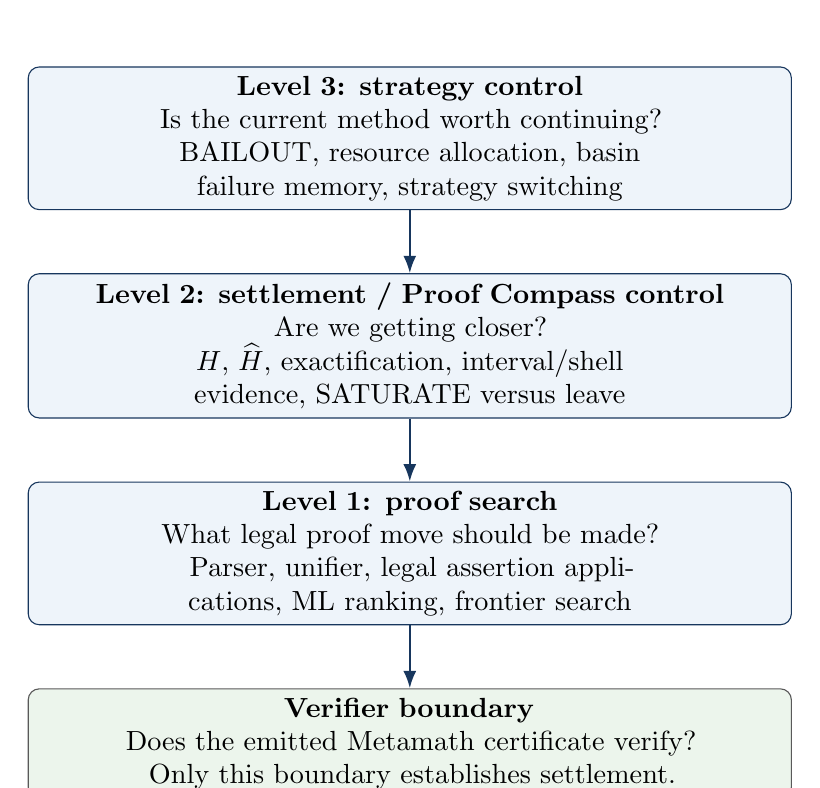
\begin{tikzpicture}[
node distance=8mm,
box/.style={rectangle,rounded corners,draw=predblue,fill=softblue,text width=0.78\textwidth,align=center,minimum height=11mm},
ver/.style={rectangle,rounded corners,draw=black!65,fill=softgreen,text width=0.78\textwidth,align=center,minimum height=11mm},
arr/.style={-{Latex[length=2.2mm]},thick,predblue}
]
\node[box] (l3) {\textbf{Level 3: strategy control}\\Is the current method worth continuing?\\BAILOUT, resource allocation, basin failure memory, strategy switching};
\node[box,below=of l3] (l2) {\textbf{Level 2: settlement / Proof Compass control}\\Are we getting closer?\\$H$, $\Hhat$, exactification, interval/shell evidence, SATURATE versus leave};
\node[box,below=of l2] (l1) {\textbf{Level 1: proof search}\\What legal proof move should be made?\\Parser, unifier, legal assertion applications, ML ranking, frontier search};
\node[ver,below=of l1] (v) {\textbf{Verifier boundary}\\Does the emitted Metamath certificate verify?\\Only this boundary establishes settlement.};
\draw[arr] (l3) -- (l2);
\draw[arr] (l2) -- (l1);
\draw[arr] (l1) -- (v);
\end{tikzpicture}
\end{center}

This hierarchy is the strongest unifying description of the late Predator line: search, then settlement assessment, then strategy assessment, with all of them subordinate to certificate verification.

\section{The branch structure rather than a fake straight line}

The surviving documentation does not justify pretending that every numerical version is a direct ancestor of the next. A more faithful high-level lineage is:

\begin{center}
\begin{tabular}{c}
\fbox{P1} $\to$ \fbox{P2} $\to$ \fbox{P3} $\to$ \fbox{P4}\\[1.0ex]
$\downarrow$\\[-0.3ex]
\fbox{P5} $\to$ \fbox{P6} $\to$ \fbox{P7} $\to$ \fbox{P7.1}\\[1.0ex]
$\Downarrow$\ \textit{reconstructed continuity}\\[0.6ex]
\fbox{8.001/8.002} $\to$ \fbox{8.015} $\to$ \fbox{8.016} $\to$ \fbox{8.017} $\to$ \fbox{8.018}\\[1.2ex]
\textit{separate experimental branch from recovered 8.x base:}\\[0.5ex]
\fbox{8.003 broad transfer} $\to$ \fbox{8.004 DCD}
\end{tabular}
\end{center}

Solid arrows denote relationships explicitly supported by the surviving descriptions. Dashed arrows denote reconstructed continuity where the exact engineering transition is not fully documented in the supplied material.

\section{Predator 8.019 - the documented next-controller proposal}

\begin{statusbox}\proposed\end{statusbox}

The 8.018 notes themselves propose a next selective controller with three ideas:
\begin{itemize}
\item adaptive utility accounting;
\item a principled choice between SATURATE and BAILOUT;
\item a portfolio of competing proof-tree basins rather than effectively one active basin at a time.
\end{itemize}

The natural state question is:
\[
\text{Which basin deserves the next unit of computation?}
\]

A basin utility may schematically take the form
\[
U(b)=\frac{\text{estimated settlement progress}+\text{certified information gain}}{\text{expected additional cost}}.
\]

The controller then chooses among
\[
\boxed{\text{SATURATE}}
\qquad
\boxed{\text{CONTINUE}}
\qquad
\boxed{\text{BAILOUT}}.
\]

In the current project direction, however, the author has elected to treat the next substantial redesign as a major version rather than continue the 8.019 numbering.

\section{Predator 9 - proposed information-rich verified search}

\begin{statusbox}\proposed\quad\textit{Current design proposal; not a historical source claim.}\end{statusbox}

Predator 9 is intended as a genuine major-version boundary. Predator 8.015--8.018 progressively added control around the recovered 8.002 search engine. Predator 9 would instead make the information state itself a first-class object.

For each live proof state $S_t$ and legal action $a$, define an online information vector
\[
I_t(a)=
(\text{syntax},\ \text{target information},\ \text{MAPQUEST geometry},\ \text{state},\ \text{memory},\ \text{history/turbulence}).
\]

The controller would use only information available before or during the live search, while keeping hindsight quantities such as exact future horizon, exact Bellman defect, and final-proof membership hidden for later evaluation or training.

A high-level Predator 9 architecture is therefore:
\[
\boxed{\text{Metamath legality}}
\to
\boxed{\text{rich online information}}
\to
\boxed{\text{fair/adaptive scheduling}}
\]
\[
\boxed{\text{verified proof}}
\to
\boxed{\text{hindsight labels for the next model}}.
\]

Potential live signals include:
\begin{itemize}
\item legal-move rank and premise relevance;
\item target-cone membership and residual obligations;
\item Hilbert/MAPQUEST coordinates and calibrated geometric residuals;
\item local branching and transposition information;
\item verified lemma reuse and BANK utility estimates;
\item basin cost/benefit history;
\item failure prefixes and turbulence measures;
\item exactification evidence where bounded certification succeeds.
\end{itemize}

The invariant inherited from the whole mature lineage remains unchanged:
\[
\boxed{\text{heuristics control discovery; the verifier controls mathematical acceptance}.}
\]

\section{Persistent design principles across the lineage}

Several principles survive repeated redesigns and should be considered part of Predator's identity rather than properties of one version.

\begin{enumerate}
\item \textbf{Verifier sovereignty.} Learned search, heuristic geometry, self-monitoring, and federation may propose or prioritize; only a verified certificate establishes theoremhood.
\item \textbf{Legality before ranking.} Candidate legality and unification should be resolved before learned ranking can truncate or prioritize candidates.
\item \textbf{Separate intrinsic difficulty from search waste.} Learning can change the amount of material explored without changing the logical depth of a theorem.
\item \textbf{Measure solve rate and effort together.} Low effort is meaningless if it is achieved by abandoning difficult targets.
\item \textbf{Compute ground truth when possible.} On bounded fragments, BFS-computed distances provide cleaner labels than imitating one recorded human proof.
\item \textbf{Reordering is safer than destructive pruning.} Removing branches can destroy proof coverage; changing their order need not.
\item \textbf{Estimated proximity is not certified proximity.} Heuristic settlement scores require independent exactification if they are to support stronger claims.
\item \textbf{Resource allocation is itself a search problem.} By 8.018 the controller is no longer only choosing proof moves; it is deciding whether a search strategy deserves more computation.
\item \textbf{Preserve negative results.} Failed pruning, failed expert iteration in a saturated fragment, duplicate-lookup hazards, and misleading proximity signals all shaped later versions.
\end{enumerate}

\section{Known reconstruction gaps}

\begin{warningbox}
The following points are intentionally left open rather than silently reconstructed.
\end{warningbox}

\begin{itemize}
\item The exact engineering transition from Predator 7.1 to the frozen 8.001 / recovered 8.002 runtime is not fully specified in the supplied PDFs.
\item The supplied material does not establish a complete history for version numbers 8.005 through 8.014.
\item Predator 8.004 DCD is documented as a proposed separate experimental branch. The surviving sources do not establish that DCD was incorporated into 8.015--8.018.
\item The 8.018 notes freeze a workflow while one experiment was still in progress. Therefore the notes establish architecture and configuration, not the final outcome of that particular run.
\item Files named ``Predator 8.5'' in the supplied set are Mathematica heart-disease classification notebooks and are not treated here as ATP versions in the Predator theorem-proving lineage.
\end{itemize}

\section{Source basis}

This reconstruction draws principally from the following supplied documents:

\begin{itemize}
\item \textit{Predator: A Trainable Automated Theorem Prover, Version 1.1}.
\item \textit{Predator\_2: Premise Selection over ZFC Set Theory}.
\item \textit{Predator\_4: Automated Theorem Proving via Premise Selection} and scaling report.
\item \textit{Predator 5: Learning a Proof-Search Policy from Computed Geodesics}.
\item \textit{Predator 7.1 Documentation and Cross-Branch Reuse Rate Theory}, especially Appendix A, ``History of Predator.''
\item \textit{Predator 8.004: Dense Closure Distillation with a Preliminary Five-Agent Certificate-Regulated ALD Topology}.
\item \textit{Predator 8.018 Reconstruction and Resume Notes: Settlement Geometry, Proof Compass Control, Self-Aware Bailout, and Selective Kitchen-Sink Roadmap}.
\end{itemize}

The summary intentionally treats those documents as the authority for historical claims. Predator 9 is separated as a present proposal rather than retroactively inserted into the historical record.

\section{Final lineage checkpoint}

The shortest faithful summary is:
\[
\begin{aligned}
\text{P1--P4}:&\quad \text{learn what information is relevant},\\
\text{P5--P6}:&\quad \text{learn which legal search moves are good},\\
\text{P7--P7.1}:&\quad \text{make that search operate on Metamath and verify certificates},\\
\text{8.001--8.002}:&\quad \text{recover the legal engine and learned move ranking},\\
\text{8.015--8.017}:&\quad \text{measure and certify local settlement progress},\\
\text{8.018}:&\quad \text{notice when strategy-level cost/benefit collapses and bail out},\\
\text{Predator 9}:&\quad \text{make all useful online information explicit and allocate computation accordingly}.
\end{aligned}
\]

\begin{keybox}
\centering
\textbf{Predator's mature design principle}\\[2mm]
Search may become more learned, geometric, reflective, cooperative, and information-rich without widening the mathematical trust boundary. The final Metamath certificate remains the authority.
\end{keybox}

\end{document}
